\section{I/O}

\textbf{Throughput-Latency Tradeoff:} $T = T_0\frac{\rho}{1-\rho}$

\textbf{Hard Disks} Each sector of a hard disk records Sector ID and data, ECC,
synchronization feilds and gaps, to access a sector you need to:
\textbf{seek(move the head), rotational latency, data transfer, controller overhead}

\textbf{Disk performance}:
$\text{seek time}+\frac{.5}{RPM/60}+\frac{sector}{TR}+\text{controller delay}$

\textbf{HW/SW IO interface} Two common approaches for this are using registers and
buffers or \textbf{Memory mapped IO}, in registers there are data registers and
command registers. In memory mapped IO portions of physical addresses are assigned
to each IO device. IO addresses correspond to device registers and buffers. IO
address space is protected so user programs cannot access it

\textbf{Physical IO interface} Common interfaces include \textbf{busses} and
\textbf{point-to-point links \& switch-based interconnects}

\textbf{Bus} A shared communication link that connects multiple IO devices, it is
a single set of wires which connect in parallel e.g. 32-bit bus = 32 wires of data.

\textbf{Bus Transactions}

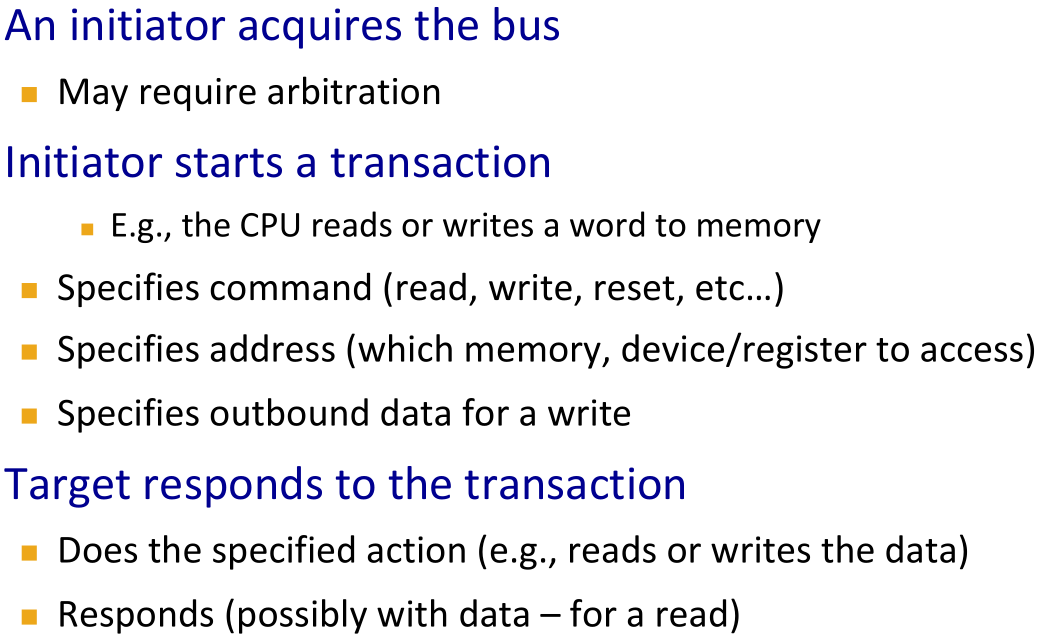
\includegraphics[width=\linewidth]{png/bustransaction.png}

\textbf{Synchronus Bus}

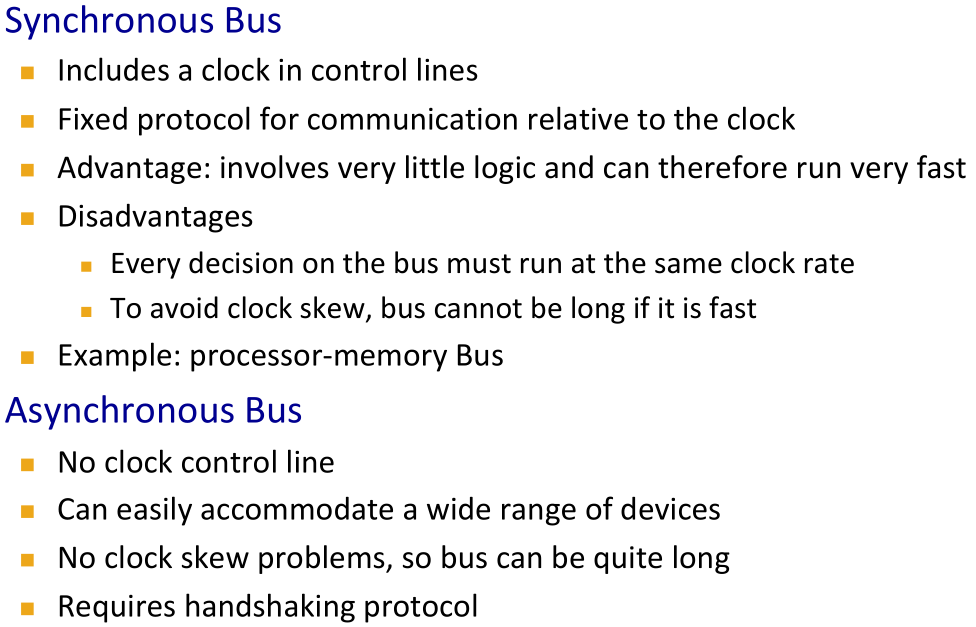
\includegraphics[width=\linewidth]{png/bus_sync.png}

\textbf{Increasing bus bandwidth} To increase bandwidth we can transfer in blocks,
transferring a burst of data. We can also pipeline the bus, we increase the clk
frequency and have mulitple lines of data in flight at once. The advantage of a
bus is that it's simple and has broadcast and is serialized, but it's slow

\textbf{Point-to-Point Links \& Switches} Allows to have multiple transactions
going on at once, an example is PCI-e. Also allows much higher clock frequencies.

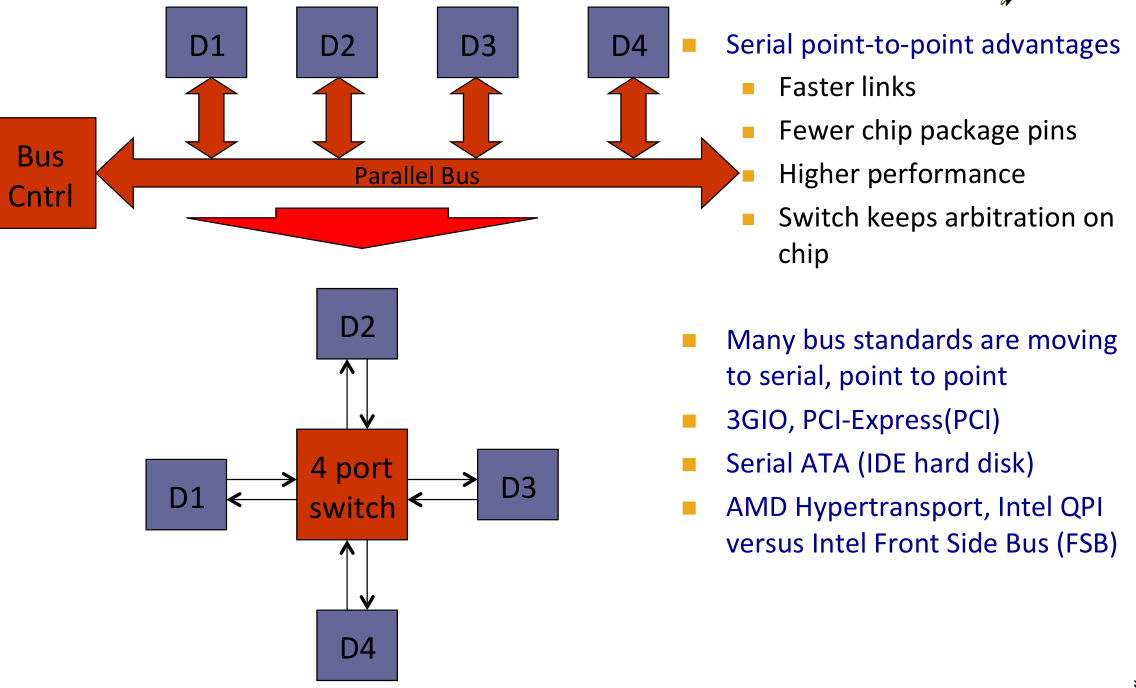
\includegraphics[width=\linewidth]{png/ptplink.png}

\textbf{IO notification w/ polling} OS periodically checks the status register

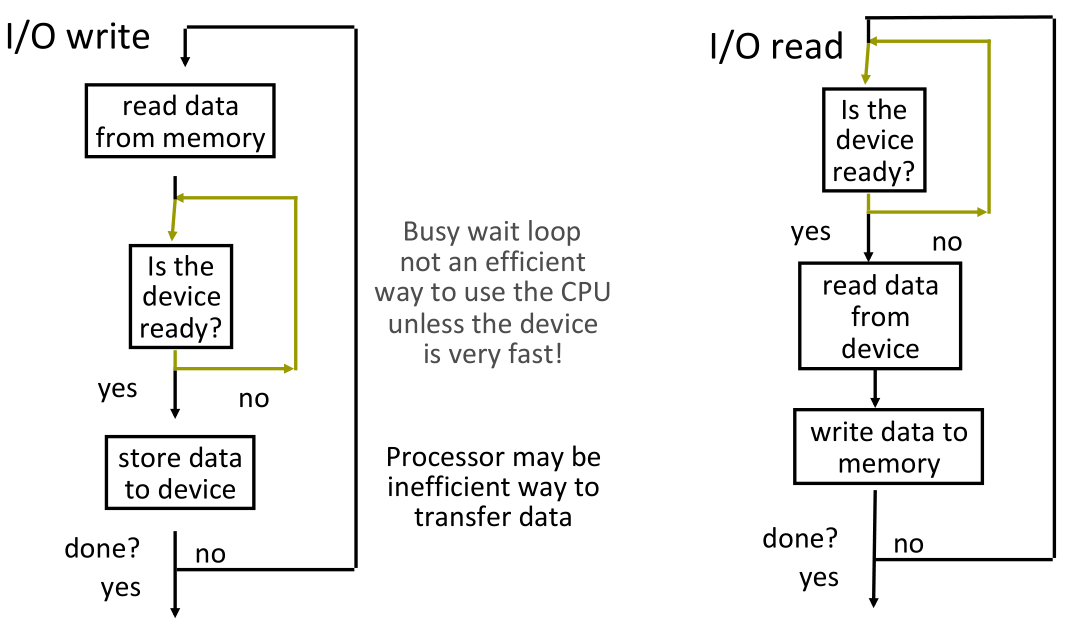
\includegraphics[width=\linewidth]{png/polling.png}

\textbf{IO notification w/ interrupts} Just like an exception but due to en external
source, execution is only halted during actual transfer.

\textbf{Direct Memory Access (DMA)} A custom engine for data movement, transfer
blocks of data to or from memory without CPU intervention. The processor sets up
DMA by giving the indentity of the device and the memory address for source/dest
DMA egines are arbiters.
